Using cognitive modelling techniques for simulating human behaviour, and limiting people interactions can save a lot of human and other resources, time and money. Therefore a variety of researchers are contributing to intelligent agents field. Beliefs, desires and intentions (BDI) constitute the core part of an intelligent agent. BDI model describes the basic characteristics of agents' mental state since the BDI logic system is easy to be implemented on the computer, and has been widely applied in the field of artificial intelligence in computer science. In recent years, many scholars have used Java, Jason or some other programming languages to implement BDI agent model on computer.

In 1987, Bratman\cite{MICHAEL_PlansResource_1988} discussed the relationship between beliefs, desires, intentions and actions as well their important roles in agent behaviours. With this paper the BDI model and BDI logic were the found. In 1991, Rao and Georgeff\cite{Michael_BDIAgency_1999} modelled the BDI agent behaviour and treated beliefs, desires and intentions as three modal operators and at the end applied BDI agent in airline traffic management. Nowadays, the research on BDI agents are not only used in high value domains but also in daily lives. There exist cases of applications of BDI agents not only in high technology industrial aspect such as airplane or space shuttle, but also in commercial field or entertainment such as robot soccer games.

The BDI model is a popular and well-studied architecture of agent for intelligent agents situated in complex and dynamic environments. The model has its roots in philosophy found in Bratman’s theory of practical reasoning\cite{Sebastian_Hierarchical_2006}. Practical reasoning involves two important processes: deciding what goals we want to achieve, and how we are going to achieve these goals. The former process is known as deliberation, the latter as means-ends reasoning\cite{Gerhard_MultiSystem_1999}. When an agent is placed in an environment, it should decide what to do and how to do it. There are a lot of options of affairs states, but not all of them are good choices. Some other affairs more or less have influences on the feasibility of achieving these goals. The deliberation process is used to understand and filter what options are available, in addition, generate the set of alternatives which will be chosen as following. These chosen options become intentions which can be treated as the outputs of deliberation. For example, if you are standing in a supermarket and very thirsty, then you are faced with a decision to choose a drink. There are a lot of options like wine, beers, milk, water and juice, however, picking up a bottle of wine is not available to you if you are younger than 18 years old. After collecting all the available options, you must choose and commit to some of them which become intentions next. Subsequently, we need the mean-ends reasoning process to plan how to achieve these intentions. Furthermore, if your intention is to buy a bottle of water, then you plan to go to the shelf with water on it, and then stretch your arm to get a bottle of water on the top. Finally, you execute this plan to get water.

As a theory of practical reasoning, BDI model has three attributes that are belief, desire and intention.

% TODO BDI three attributes
Beliefs represent the informational state of the agent and are updated appropriately after each sensing action. They may be implemented as a variable, a database, a set of logical expressions, or some other data structure\cite{Rao_BDITheory_1995}. Belief means how the agent look at the world and it is the basis of BDI model. Belief includes the information about environment, other agents and itself. An agent needs to be allowed to update its beliefs at any time. Updating information comes from the perception of the environment, and the execution of intentions. An agent can use sensors to perceive the environment to get signals to believe. In addition, after executing some intentions, they become the information believed by the agent. Belief is not the same concept as knowledge. Beliefs are only required to provide information on the likely state of the environment, but knowledge is the realisation of a fact. Beliefs are just the state believed by agents but no one can ensure what their beliefs are true. Simply saying, knowledge is true belief.

Desires represent the motivational state of the agent\cite{Rao_BDITheory_1995}. They represent objectives or situations that the agent would like to accomplish or bring about. They are states of affairs that the agent would wish to bring about or to keep. Desires may be achieved or never achieved, and it is not necessary to believe that desires must be achieved. Desires are different from goals although they look pretty similar. Desires can be inconsistent and the agent doesn't need to know the means of achieving these desires. Desires have the tendency to 'tug' the agent in different directions. They are inputs to the agent's deliberation process, which results in the agent choosing a subset of desires that are both consistent and achievable. Such consistent and achievable desires are usually called goals\cite{Gerhard_MultiSystem_1999}. For example, sleeping and working may be both my desires, but they can not be my goals at the same time because they have conflicts.

Intentions are desires or actions that the agent has committed to achieve\cite{Alejandro_LearnBDI_2004}. Intentions are stronger than desires. Desires are just wishes that may be achieved or may be not, but intentions to an extent are decided to be achieved. Michael Wooldridge in \cite{Gerhard_MultiSystem_1999} concluded four roles of intentions in practical reasoning. The roles are: intentions drive means-ends reasoning; intentions constrain future deliberation; intentions persist and intentions influence beliefs upon which future practical reasoning is based. Intentions driving means-ends reasoning means that intentions have decisive influences on actions the agent will execute. Agents are expected to determine ways of achieving intentions. Intentions constraining future deliberation means that options that are inconsistent with this intention will not be considered. Intentions persisting means that intentions will never be given up unless the reason is rational. As we know, intentions are committed desires which can not be easily abandoned. For if I immediately drop my intentions without devoting resources to achieving them, then I will never achieve anything\cite{Gerhard_MultiSystem_1999}. But when a good reason exists, I still can drop intentions instead of persisting them for a long time without achievement. If it is very clear that the intentions will never been achieved, then there is no need to keep them. Similarly, if the reason for intention is no longer true, then intentions should be given up. Another reason of dropping intentions is the intentions have been achieved already. Intentions influencing beliefs upon which future practical reasoning is based means that believed intentions will be achieved. If I adopt an intention, then I can plan for the future on the assumption that I will achieve the intention. For if I intend to achieve some state of affairs while simultaneously believing that I will not achieve it, then I am being irrational\cite{Gerhard_MultiSystem_1999}. Agents should believe that they believe there is at least some way that the intentions could be brought about and believe that under "normal circumstances" agents will succeed with the intentions, or say it in another way, agents do not believe they will not bring about their intentions. Generally speaking, intentions are not random ideas, but the wants to a reasonable extent. It plays an important role in BDI model that leading to actions, constraining future deliberation and influencing future beliefs. Specifically, the agents should drop off some intentions at times to avoid resource wasting. It is necessary to keep a good balance between these different concerns.
\todo{For some reason, the spacing here between paragraphs seems to increase at times. I haven't quite figured out why and when this happens.}

Beliefs, desires and intentions are three attributes of BDI model and constitute the foundation of BDI agents. While some other components building connection between beliefs, desires and intentions are also indispensable to implement BDI agents and make the BDI architecture completed.
% TODO BDI basic architecture//pic
Several basic components can be found in the following figure, which is a brief BDI architecture. A variety of BDI agents have been designed to fit the unstable environment and to complete all sorts of tasks. Different BDI agents have different architectures, but their core ideas are same.

\begin{figure}[htbp]
  \centering
  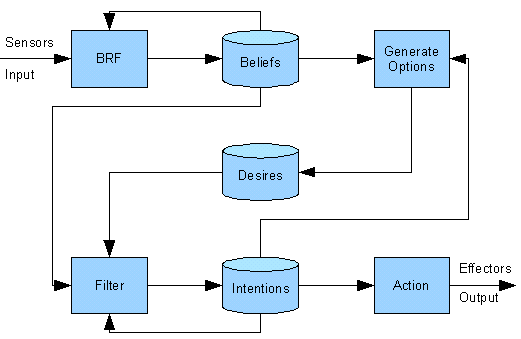
\includegraphics[width=\textwidth]{images/BDIAr}
  \caption{Brief BDI architecture \cite{BDIA}}%use cite instead
  \label{fig:Brief BDI architecture}
\end{figure}

The sensors of the BDI agent perceive the environment and convert the perceptions to signals as the inputs to the belief revision function. It will collect the perceptions from outside as well as the beliefs which are stored in the beliefs set. After mapping the information, computing and revising using belief revision function, the new beliefs will set into the beliefs set. The belief revision function prefers minimal change rather than modifying a lot. There are not big differences between the revised beliefs set and the previous one to preserve as much information as possible by the change\cite{Antje_SpatialBelief_2011}. The belief revision function is used to keep the beliefs set being updated to fit the unstable environment, on the other hand, it can avoid the inconsistent situations occurring among those beliefs like the agent believes what it does not believe.

The beliefs set contains information about the current environment which the agent has. The data in beliefs set may be sentences, rules or some other manifestations. In the AGM (named after the names of their proponents, Alchourrón, Gärdenfors, and Makinson)\cite{alchourron_revision_1985} approach, an agent’s beliefs are modeled by a deductively closed set of formulas called a belief set\cite{James_revise_2011}.
The current set of beliefs is represented by a deductively closed set of logical formulae K called belief base, the new piece of information is a logical formula P, and revision is performed by a binary operator * that takes as its operands the current beliefs and the new information and produces as a result a belief base representing the result of the revision\cite{M_Belief}. Many researchers are doing researches in belief revision using AGM approach.
The option generator reads the beliefs information and returns a list of options which are current desires into the desires set. It determines the desires depending on the agent’s current beliefs and current intentions. The desires set contains many desires are possible courses of actions available to the agent, and These desires can be no matter achieved or not. The filter determines the agent’s intentions depending on current beliefs, desires, and intentions. It needs to consider about more situations than the functions in previous steps. Desires will become more rational after filtering.

The intentions set stores the agent’s current focus, which are going to be executed or committed to be executed at some time. Once an intention is adopted, it should not be immediately dropped out because of the commitment. But in some situations, the intentions should be given up depending on  three commitment strategies having been proposed in Rao and Georgeff’s work:  blind, single minded and open minded. A blindly committed agent is an agent who maintains his intentions until he believes that he has achieved them. A single minded committed agent is an agent who maintains his intentions as long as he believes that they are still options. An open minded committed agent is an agent who maintains his intentions as long as they are still goals\cite{Roberto_BDIATL_2005}. The action selection function determines the actions to perform depending on current intentions. We would achieve nothing if we just have intentions instead of knowing how to do it. Normally, there is a plan library of mapping between the intentions and actions. The intentions go through the planner and the actions which mapping the corresponding intentions are founded. At last, a plan of how to achieve the intentions come out and the agent will execute these actions.

For understanding the relationships between the seven main components of BDI agent architecture, one table is presented as followed:

\begin{table}[!hbp]
  \label{tab:BDIC}
  \begin{tabularx}{\textwidth}{|l|p{5cm}| >{$}X<{$} |}
  \hline
  \textbf{Component} & \textbf{Meaning} & \textbf{Formalisation} \\
    \hline
    Beliefs set & Information about the current environment which the agent has & B \\
    \hline
    Belief revision function & determines a new set of beliefs depending on perceptual inputs and the agent’s current beliefs & B \times P \to B\\
    \hline
    Options & determines desires depending on the agent’s current beliefs & B \times I \to D \\
    \hline
    Desires set & possible courses of actions available to the agent & D \\
    \hline
    Filter & determines the agent’s intentions depending on current beliefs, desires, and intentions & B \times I \times D \to I \\
    \hline
    Intentions set & the agent’s current focus & I \\
    \hline
    Action selection function & determines an action to perform depending on current intentions & I \to A  \\
    \hline
  \end{tabularx}
  \caption{Components of brief BDI agent architecture}
\end{table}

This table shows the order of using the seven components of BDI architecture as well as giving the formulas of each function. There, $Bel$ is a set of all possible beliefs, $Des$ is a set of all possible desires and $Int$ is a set of all possible intentions. Therefore, an agent state can be presented as $(B,D,I)$ with $B \subseteq Bel, D \subseteq  Des, I \subseteq  Int$. $P$ is a set of current perception which are obtained by the sensors of the agent. we can understand the the process of BDI agent working better through seeing this table. Firstly, $B$ has stored some beliefs which are read by BRF while it getting the perception from the sensors. After operating BRF, some of beliefs are removed, some are added, some are modified and so on. So the new beliefs set $B$ built on basis of $P$ and original $B$. Subsequently, Options use the new $B$ and current Intentions set $I$ to determine the desires set $D$ and store it. Moreover, the filter select intentions by referencing $B,D,I$, then the new intentions set comes out. Finally, the action selection function makes a plan to execute actions to achieve $I$.

The process of $B \times P \to B$, $B \times I \to D$ and $B \times I \times D \to I$ belongs to deliberation. They are deliberated in-depth gradually and the range of intentions are narrowed, especially the filter which should consider of all there datasets. At last, the intentions are limited in particular ranges. The plans will be made more effective and more targeted.  $I \to A $ can be treated as the process of means-ends reasoning, whose output is planning. $B,D I$ are connected to function parts instead of connecting to each other directly. They are just databases and need rules or mechanism to help them execute actions.

% TODO BDI applications (short)
With the increasing needs of intelligent agents, more and more applications base on BDI model are applied in our life. PRS and dMARS are both BDI-based systems for the reaction control system of the NASA Space Shuttle Discovery. Additionally, an air-traffic management system, OASIS, is well-known as a BDI-dased agent. The system architecture for OASIS is made up of one aircraft agent for each arriving aircraft and a number of global agents including a sequencer wind modeller coordinator and trajectory checker\cite{Rao_BDITheory_1995}. Furthermore, robot soccer which are designed using BDI model becomes very popular in universities. We can feel that, BDI agents bring many profits to human beings, they make the life more convenient. However, it still has development space in this field.

Although the BDI model is developed during about 30 years, some obstacles are not overcome and some challenges are still there. Most BDI implementations do not have an explicit representation of goals. The agents should reason the goals from the current beliefs and intentions. Besides, the BDI model contains three attributes, beliefs, desires and intentions. In some situations, not all the three attributes are needed. Sometimes, an agent collect the beliefs and jump to intentions directly without desires. However, for some distributed multi-agents, just three attributes are not sufficient to execute the actions.  Furthermore, the agents in the multi-agents system do not have an explicit mechanism for interaction and integration among them. When an increasing number of agents join the system, the interaction with each agent will be more and more difficult. As an intelligent agent, the BDI agent do not have a good ability to learning from from past behavior or other agents’ behavior. So that the rate of development will not be high if lack mechanisms to learn from others. However, BDI model has its own advantages. Beliefs, desires and intentions are similar to the mental activities of human beings. Therefore, it is not easy to construct the logics or mechanisms for it. With the wildly used of computers and mobile devices, the situation of multi-agent interaction will be better. As many computer languages and logic languages are grasped by more people, the BDI agent will bring human beings more surprises.

An introduction of beliefs, desires and intentions model is presented in this section. The BDI agent belongs to intelligent agent which are autonomous, computational entities. The BDI agent executes actions on the basis of BDI model that containing three main attributes which have close relationship with each other. The brief BDI agent architecture is a clear description of process of BDI agents work. And They follows the practical reasoning theory. Different BDI implements show different architectures, but the core idea of these agents are still beliefs, desires and intentions. With an increasing number of BDI applications go into the humans life, more challenges come up too. The BDI model has its own advantages and disadvantages, but I still believe that it can bring more surprises to own life in the future.



